\chapter{Introduction}
\label{introduction}

As robots become cheaper and more popular for common tasks, they are frequently used as independent
platforms without significant supporting infrastructure or personnel. Because of this, it is
important that robots are equipped with easy to use interfaces to control them and diagnose problems.
Touchscreen displays are ideal for this use case, as they can be attached to any even surface and do
not require any specialized input devices.

This thesis implements an example of such an interface as a standalone microcontroller board
that can be directly attached to a robot built on the \textit{Wolfgang} robot platform (see section
\ref{introduction/motivation} for more details). It can be used to debug common issues with the devices
used by the robot, such as connectivity or misconfiguration.

This introduction gives a brief motivation for this bachelor thesis in section \ref{introduction/motivation}.
Since the \textit{Wolfgang} robot platform is used for the \href{https://www.robocup.org/}{\textit{RoboCup}}
competition, it is explained in section \ref{introduction/robocup}. Section \ref{introduction/thesis-goal}
defines the goals of the thesis.

Chapter \ref{related-work} presents related work in robot interface design, focusing on robots
designed for frequent interaction with humans. After that, chapter \ref{basics} explains some basics
as well as the bus and protocol used by the implementation. Next, chapter \ref{implementation}
describes the actual implementation and rationale behind important design decisions. Chapter \ref{evaluation}
then provides a short overview of the usability of the finished work and relevant benchmarks while
chapter \ref{discussion} discusses these results. Finally, Chapter \ref{conclusion-and-future-work}
summarizes the findings and lists possible improvements to the current implementation.

\section{Motivation}
\label{introduction/motivation}

The work done in this thesis is primarily intended for use with the \textit{Wolfgang} robot platform
used by the \textit{RoboCup} team \textit{Hamburg Bit-Bots}. It consists of various devices~\cite{bit-bots-specs}
that communicate using the \textit{ROBOTIS Dynamixel Protocol 2.0}~\cite{dynamixel-protocol-2} over
an \textit{RS-485} or TTL bus.

Without a computer connected to the robot, it is not possible to monitor the status of the connected
devices. Devices may be unreachable for different reasons:

\begin{itemize}
    \item the device is physically disconnected
    \item the device is powered off or otherwise malfunctioning
    \item the device's packets are lost, either due to interference or a misbehaving bus participant
    \item the device never sends any packet because it is waiting for another device that is not sending
          for one of the reasons above
\end{itemize}

\begin{figure}[h]
    \centering
    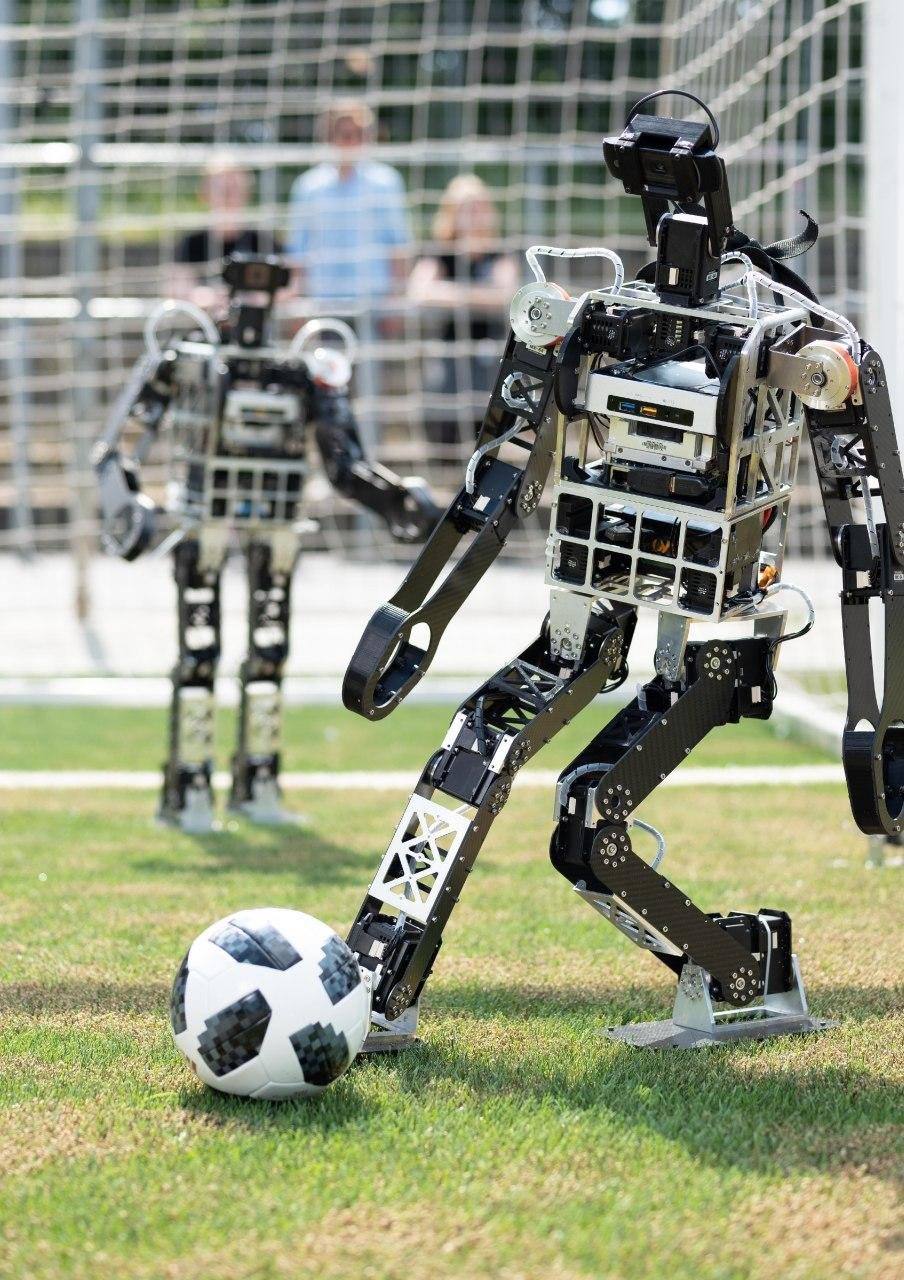
\includegraphics[scale=0.75]{img/wolfgang.jpg}
    \caption{The \textit{Wolfgang} robot platform}
\end{figure}

While it is always possible to connect a computer in case of an obvious malfunction, this is a
significant amount of overhead. It does not allow for quick detection of disconnected devices
or anomalous readings of a single device. In a competition like \textit{RoboCup}, it is important
to quickly detect problems in order to fix them in the field. Noncritical errors may not disable
the robot but they can still have an impact on its performance in a game.

Due to the extensible nature of the protocol, other robot platforms using the same protocol and
a bus compatible with a UART (Universal Asynchronous Receiver Transmitter) interface would also
work, with code changes only required for adding support for new device models.

\section{RoboCup}
\label{introduction/robocup}

\textit{RoboCup} (\url{https://www.robocup.org/}) is a competition designed to promote robotics and
AI research. It intends to set challenges that are both technically difficult and socially impactful.
The long term goal is to create fully autonomous robots that can play soccer and win against the
current winners of the FIFA World Cup championship~\cite{robocup-objective}.

\begin{figure}[h]
    \centering
    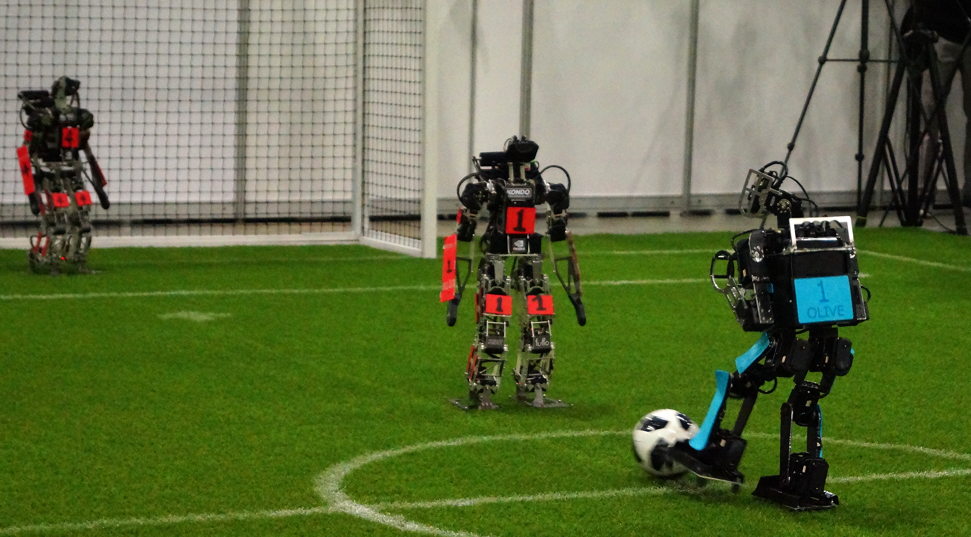
\includegraphics[scale=1.5]{img/robocup_game.png}
    \caption{A \textit{RoboCup} soccer game}
\end{figure}

While soccer was the original idea behind \textit{RoboCup}~\cite{robocup-history}, there are now many
different categories that focus on specific challenges:

\begin{itemize}
    \item \textit{RoboCupSoccer}
    \item \textit{RoboCupRescue}
    \item \textit{RoboCup@Home}
    \item \textit{RoboCupIndustrial}
    \item \textit{RoboCupJunior}
\end{itemize}

The leagues in each category are based on the physical layout of the robot or the specific task. For
example, the \textit{RoboCupSoccer} category~\cite{robocup-soccer} includes the following leagues:

\begin{itemize}
    \item \textit{Humanoid}
    \item \textit{Standard Platform}
    \item \textit{Middle Size}
    \item \textit{Small Size}
    \item \textit{Simulation}
\end{itemize}

The \textit{Hamburg Bit-Bots} team competes in the \textit{Humanoid} league (\textit{KidSize} and
\textit{TeenSize}) with robots built on the \textit{Wolfgang} robot platform~\cite{robocup-humanoid-teams}.

By defining clear rules and goals, the various \textit{RoboCup} leagues make it possible to compare
and evaluate different approaches in both robotics and AI research. They also make research in these
areas more visible to the general public.

\section{Thesis Goal}
\label{introduction/thesis-goal}

The goal of this thesis is to determine a suitable microcontroller board and develop
the required firmware for

\begin{itemize}
    \item collecting status information of the connected devices by passively listening on the bus~\dots
    \item displaying this information on an integrated touchscreen display and~\dots
    \item navigating between detailed views for each device/model using the touchscreen
\end{itemize}

In particular, it should be possible to identify unreachable or disconnected devices at a glance.
Adding support for new device models should be easy and effortless.

Both display and microcontroller should be compact enough to be able to attach and detach them
from a robot quickly.
